\newpage

\section{Detekcja twarzy} \label{section:face_detection}

W przetwarzaniu cyfrowym obrazu stosujemy technikę od ogółu do szczegółu. Przykładowo chcąc uzyskać barwę nadwodzia najpierw musimy wykryć samochód itp. W pracy dyplomowej by uzyskać informacje o oczach czy ustach potrzebujemy najpierw informacji o wystąpieniu twarzy i gdzie się ona znajduje. Dlatego pierwszym etapem przetwarzania jest detekcja ludzkiej twarzy. Chcemy z obrazu uzyskać informację o jej położeniu i w następnych etapach operować tylko na wycinku zdjęcia. 

\subsection{Algorytmy detekcji twarzy}

Na potrzeby projektu zostanie zaimplementowane pięć algorytmów, których celem jest wykrycie twarzy na zdjęciu. Krótki opis poszczególnych metod znajduje się w następnym podrozdziale. Z zaproponowanych rozwiązań zostanie finalnie wybrane jedno po serii badań i testów mających na celu wybór zarówno skutecznego jak i szybkiego.

\subsubsection{Klasyfikator kaskadowy} \label{section:face_casacde_classifier}
\textit{Cascade Classifier} to jedno z podejść do zadania klasyfikacji obiektów. Kaskadowość przejawia się tym, że klasyfikator składa się z łańcucha mniejszych klasyfikatorów. Z danych wejściowych jednego może korzystać następnym jako dodatkowe źródło informacji i użyć je do własnej klasyfikacji. Z tego powodu kolejne elementy są bardziej zaawansowane i operują na większym zestawie danych. Dzięki swojej kaskadowej naturze modele takie mogą być lepiej trenowane i dawać lepsze rezultaty niż klasyfikatory typu monolity.

\vspace{5mm}

Do ładowania i przetwarzania kaskadowych klasyfikatorów w projekcie zostanie użyty moduł \textit{CascadeClassifier} \cite{cascade_opencv} biblioteki \textit{OpenCV} \cite{opencv}. 

\paragraph{Haar}

Jednym z najbardziej znanych modeli klasyfikacji kaskadowej jest \textit{Haar}, który został opisany po raz pierwszy w 2001 roku \cite{haar_proceeding}. Może on być używany do klasyfikacji różnych obiektów, ale autorzy skupiali się głównie na detekcji twarzy. Algorytm \cite{haar_towards} \cite{haar_pyimage} \cite{OBUKHOV2011517} bazuje na podzieleniu zdjęcia na regiony i wykorzystaniu w każdej z nich pięciu cech krawędzi (patrz \hyperref[{fig:haar_features}]{\textit{rysunek \ref{fig:haar_features}}}). Algorytm porównując jasność pikseli w białej i czarnej części stwierdza czy istnieją krawędzie lub linie. Cechy składające się tylko z dwóch regionów odpowiadają za wykrycie pionowych i poziomych krawędzi. Zestaw trzech za wykrycie linii. Natomiast kwadratowa cecha za zmiany przekątne. W dzisiejszych czasach \textit{Haar} nie jest już tak często stosowany jak jeszcze parę lat temu.

\begin{figure}[!h]
    \begin{center}
        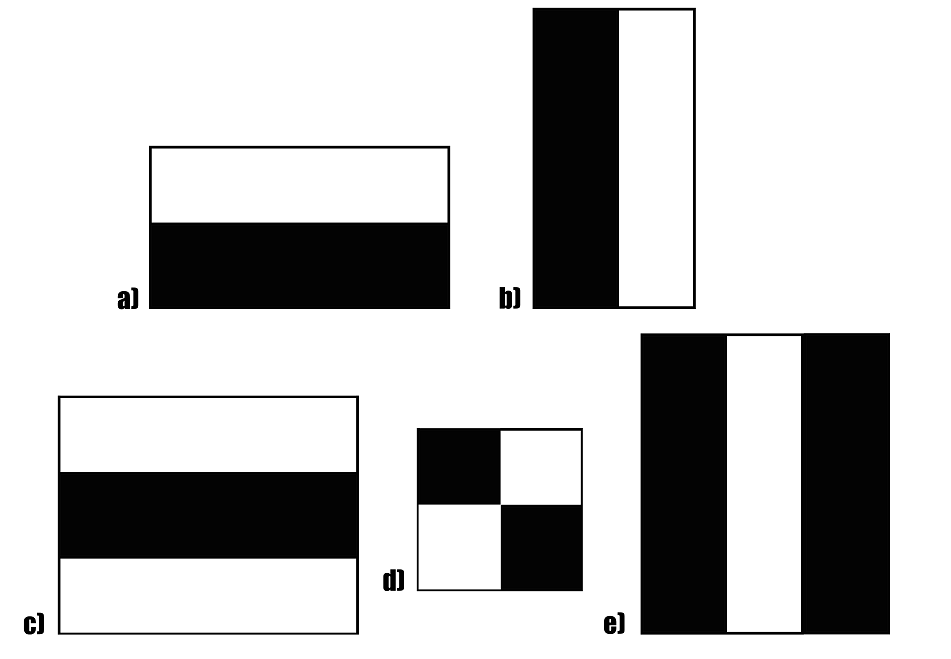
\includegraphics[scale=0.2]{img/face_section/haar_features.png}
        \caption{Obliczane cechy w modelu Haar. Źródło: \cite{haar_towards}}
        \label{fig:haar_features}
    \end{center}
\end{figure}

Na potrzeby pracy dyplomowej zostanie wykorzystany model \textit{Haarcascade Frontalface Default} \cite{haar_frontal} autorstwa Rainera Lienharta.



\paragraph{Local binary patterns}
Metoda ta porównuje piksele z ośmioma swoimi najbliższymi sąsiadami w ustalonej kolejności. Jeśli jasność głównego piksela jest większa niż porównywanego to na odpowiedniej pozycji 8-bitowej liczby wstawia 1, inaczej 0. Następnie z uzyskanych w ten sposób liczb tworzy histogram używany jako deskryptor cech. Take dane mogą być użyte do uczenia maszynowego. \cite{comp_haar_lbp}
\par
Jest to metoda cechująca się wysoką szybkością działania i z tego powodu stosowana w systemach z ograniczonymi zasobami sprzętowymi. Niestety kosztem efektywności.
\par
W projekcie użyty będzie model \textit{LBP Cascade Frontalface} \cite{lbp_xml}.


\subsubsection{Histogram zorientowanych gradientów}
Metoda \textit{HOG (Histograms of Oriented Gradients)} \cite{hog_article} została opracowana kilkanaście lat temu przez Navneet Dalal i Bill Triggs celem detekcji ludzkiego ciała. Aktualnie, mimo upływu lat, jest wciąż szeroko wykorzystywana do klasyfikacji obrazów czy wykrywania twarzy.
\par
Uzyskanie histogramu HOG składa się z kilku etapów. Metoda \cite{hog_wprowadzenie} \cite{learnopencv_HOG} \cite{guide_hog} ta bazuje na obliczeniu gradientów poziomych i pionowych. Możliwe jest to przez filtrowanie za pomocą odpowiedniego jądra lub przez operator Sobela \cite{feature_extraction}. Dla tak wyodrębnionych gradientów oblicza się ich długość i kierunek (kąt). Następnie dzielimy zdjęcie na obszary o wielkości $8x8$. Dla każdego regionu tworzymy jednowymiarowy wektor o 9 komórkach, w których będzie zapisany histogram HOG. Pola wektora odzwierciedlają kierunek gradientu i odpowiadają kolejnym wielokrotnościom kąta $\measuredangle 20 ^{\circ}$. Wypełniamy go dodając do pól odpowiadającym danemu kątowi wartość gradientu kolejnych pikseli. Jeśli kierunek znajduje się pomiędzy dwoma kątami to wartość dzieli się zależnie od różnicy między dwiema komórkami. Celem wyeliminowania wpływu jasności i oświetlenia przeprowadza się normalizację wartości. Gdy obliczy się już histogram dla każdego regionu, łączy się je w wektor deskryptora cech HOG. Tak uzyskany wektor możemy wykorzystać jako dane uczące algorytmów klasyfikujących. W przypadku metody HOG często wykorzystuje się \textit{maszynę wektorów nośnych (SVM)} \cite{svm_toward_science}.

\vspace{5mm}

W projekcie zostanie użyta metoda \textit{HOG} z biblioteki \textit{dlib}, która uczona była z użyciem liniowego \textit{SVM}.


\subsubsection{CNN + MMOD}
Konwolucyjne sieci neuronowe (CNN) uczą się jakie cechy obrazu pozwalają sklasyfikować widoczne na nim obiekty. Za pomocą operacji splotowych, nakładając odpowiednie filtr są wstanie je uwypuklić i uzyskać istotne informacje. To właśnie w warstwie konwolucyjnej używane są odpowiednie jądra. Sieć przez trening sama dobiera optymalne filtry oraz ich wartości. Dodatkowo istnieją tutaj warstwy próbkowania (downsampling), których celem jest zmniejszenie wielkości obrazu przez pominięcie części pikseli. Pomaga to uprościć sieć, ale kosztem utraty pewnej ilości informacji. Czasem zamiast pomijać piksele brane są wartości uśredniane lub maksymalne z pewnego sąsiedztwa. \cite{jak_cnn}

\vspace{5mm}
W bibliotece \textit{dlib} sieć CNN często jest zestawiona z metodą \textit{Max-Margin Object Detection (MMMOD)} \cite{mmod}. Służy ona do optymalizacji i zwiększenia prędkości detekcji obiektów.
\par
Taka implementacja CNN+MMOD dostępna w dlib zostanie użyta w projekcie.



\subsubsection{Głębokie sieci neuronowe}


Głębokie sieci neuronowe (DNN) różnią się od klasycznych tym, że mają większą liczbę warstw ukrytych. Taki algorytm tworzy plamki o ustalonej wielkości ze zdjęć wejściowych, a następnie przepuszcza je przez kolejne warstwy sieci celem wykrycia pożądanych obiektów. Na wyjściu podaje prawdopodobieństwo, że na obrazie znajduje się interesujący nas element.
\par
W projekcie zostanie wykorzystany do tego jeden z modułów biblioteki \textit{OpenCV} zawierający implementację DNN \cite{opencv_dnn}
\par
Jednym z modeli dostępnych do detekcji twarzy przy pomocy głębokich sieci neuronowych są modele Caffe (\textit{Convolutional Architecture for Fast Feature Embedding}) \cite{jia2014caffe}. W~projekcie zostanie użyty wzorzec caffe \textit{res10{\_}300x300{\_}ssd{\_}iter{\_}140000{\_}fp16} \cite{caffemodel_res10}.


\subsection{Filtrowanie wyników}
\label{section:face_detection_filter}

Użyte algorytmy mogą dawać w wyniku błędnie określone obszary twarzy. Z tego względu zwróconą tablicę obszarów poddaję filtrowaniu.

\par
Proces ten składa się z następujących etapów:

\begin{itemize}
    \item Na początku odrzucam obszary, których środek znajduje się poza ustalonym pionowym obszarem (przyjąłem przedział [0.25, 0.75] szerokości). Wynika to z założeń, że osoba używająca telefonu, korzysta z niego patrząc na wprost, a nie z boku. Natomiast odchył od pionu to indywidualne preferencje - dlatego nie określam poziomego obszaru. (patrz \hyperref[{fig:face_boundary}]{\textit{Rysunek \ref{fig:face_boundary}}})

    \begin{figure}[!h]
        \begin{center}
            \subfigure[Przed filtrowaniem zależnym od położenia]{\label{fig:face_boundary_before}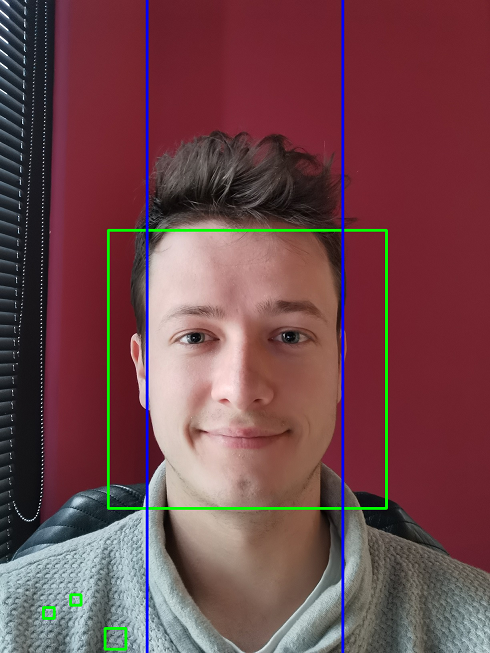
\includegraphics[scale=0.3]{img/face_section/face_filter_boundary_1.png}}
            \hspace{8mm}
            \subfigure[Po filtrowaniu]{\label{fig:face_boundary_after}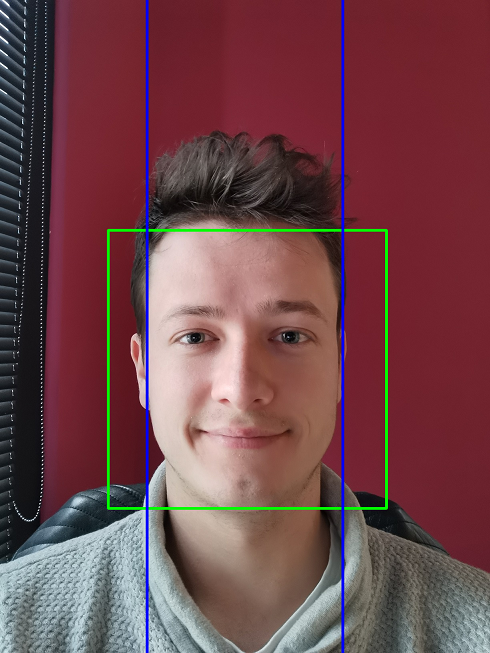
\includegraphics[scale=0.3]{img/face_section/face_filter_boundary_2.png}}
        \end{center}
        \caption{Działanie filtrowania detekcji twarzy w oparciu o położenie twarzy w centralnej części zdjęcia.}
        \label{fig:face_boundary}
    \end{figure}
    
    \item Kolejnym etapem jest odrzucenie tych detekcji, które wychodzą zbyt daleko poza zdjęcie. Jeśli którykolwiek z boków prostokąta wystaje pionowo/poziomo o odległość większą niż $10\%$ odpowiednio wysokości/szerokości to zostaje odrzucony. (patrz \hyperref[{fig:face_out}]{\textit{Rysunek \ref{fig:face_out}}})
    
    \begin{figure}[!h]
        \begin{center}
            \subfigure[Przed filtrowaniem zależnym od wystawania poza obraz]{\label{fig:face_out_before}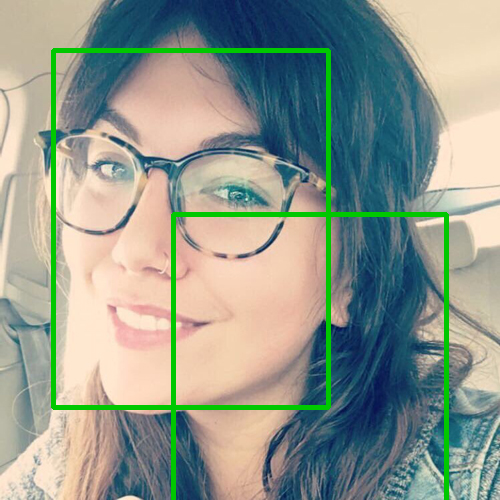
\includegraphics[scale=0.25]{img/face_section/face_filter_out_before.png}}
            \hspace{8mm}
            \subfigure[Po filtrowaniu]{\label{fig:face_out_after}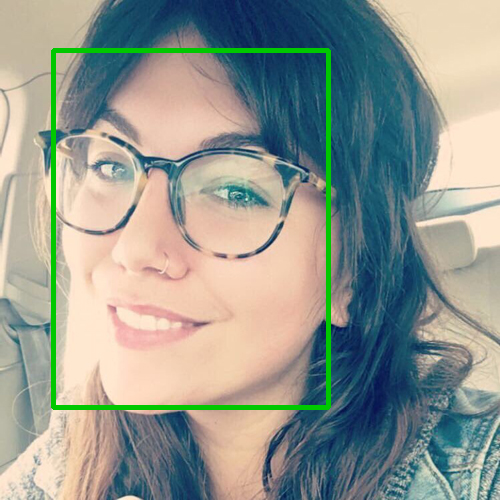
\includegraphics[scale=0.25]{img/face_section/face_filter_out_after.png}}
        \end{center}
        \caption{Działanie filtrowania detekcji twarzy w oparciu o odległość wykrytego obszaru poza zdjęcie.}
        \label{fig:face_out}
    \end{figure}
    
    \item Z pozostałych obszarów wybieram ten, który zajmuje największą powierzchnię. Taki wybór motywuję własnymi obserwacjami zachowania algorytmów detekcji twarzy oraz tym, że głowa użytkownika telefonu na obrazie z kamery przedniej zajmuje większą część płaszczyzny, ponieważ korzystając z urządzenia nie trzymamy go bardzo daleko od siebie. (patrz \hyperref[{fig:face_size}]{\textit{Rysunek \ref{fig:face_size}}})
    
    \begin{figure}[!h]
        \begin{center}
            \subfigure[Przed filtrowaniem zależnym od wielkości]{\label{fig:face_size_before}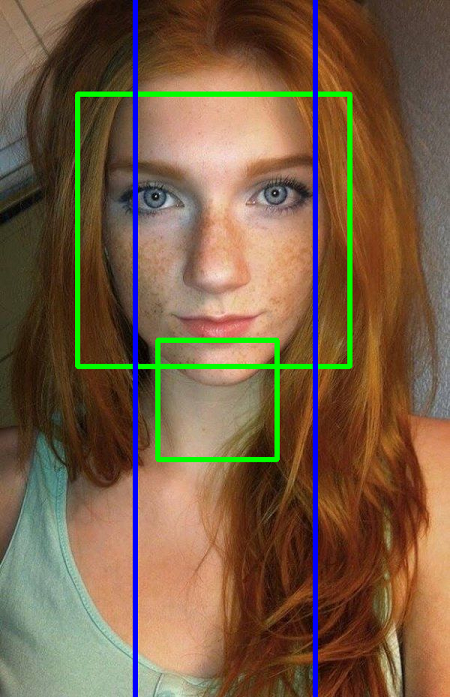
\includegraphics[scale=0.3]{img/face_section/face_filter_size_1.png}}
            \hspace{8mm}
            \subfigure[Po filtrowaniu]{\label{fig:face_size_after}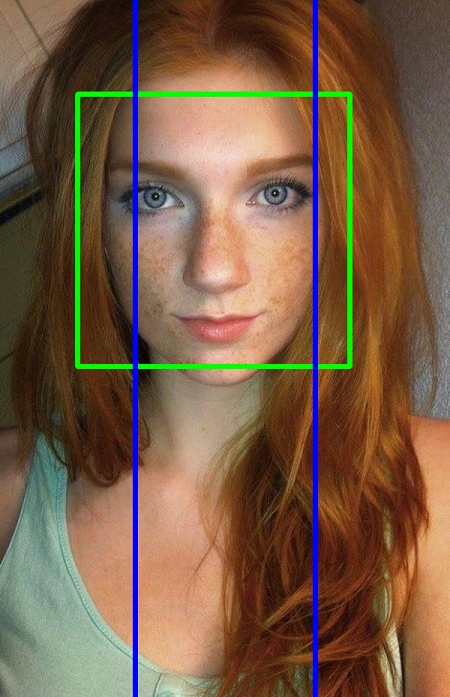
\includegraphics[scale=0.3]{img/face_section/face_filter_size_2.png}}
        \end{center}
        \caption{Działanie filtrowania detekcji twarzy w oparciu o wielkość wykrytego obszaru. Źródło zdj.: \cite{readheadPortrait1}}
        \label{fig:face_size}
    \end{figure}
    
    
    
\end{itemize}